% Hlavicka pro protokoly z fyzikalniho praktika.
% Verze pro: LaTeX
% Verze hlavicky: 22. 2. 2007
% Autor: Ustav fyziky kondenzovanych latek
% Ke stazeni: www.physics.muni.cz/ufkl/Vyuka/
% Licence: volne k pouziti, nejlepe k vcasnemu odevzdani protokolu z Vaseho mereni.


\documentclass[czech,11pt,a4paper]{article}
\usepackage[T1]{fontenc}
\usepackage{graphicx}
\usepackage{mathtools}
\usepackage{amssymb}
\usepackage{amsthm}
\usepackage{thmtools}
\usepackage{xcolor}
\usepackage{nameref}
\usepackage{babel}
\usepackage{hyperref}
\usepackage{multicol}
\usepackage[export]{adjustbox}
\usepackage{subcaption}
\usepackage{caption}
\usepackage{multirow}
\usepackage{float}
\usepackage{placeins}




%%% Nemente:
\usepackage[margin=2cm]{geometry}
\newtoks\jmenopraktika \newtoks\jmeno \newtoks\datum
\newtoks\obor \newtoks\skupina \newtoks\rocnik \newtoks\semestr
\newtoks\cisloulohy \newtoks\jmenoulohy
\newtoks\tlak \newtoks\teplota \newtoks\vlhkost
%%% Nemente - konec.


%%%%%%%%%%% Doplnte pozadovane polozky:

\jmenopraktika={Fyzikální praktikum 2}  % nahradte jmenem vaseho predmetu
\jmeno={Teodor Duraković}            % nahradte jmenem mericiho
\datum={30.~září 2024}        % nahradte datem mereni ulohy
\obor={F}                     % nahradte zkratkou vami studovaneho oboru
\skupina={Po 14:00}            % nahradte dobou vyuky vasi seminarni skupiny
\rocnik={II}                  % nahradte rocnikem, ve kterem studujete
\semestr={III}                 % nahradte semestrem, ve kterem studujete

\cisloulohy={12}               % nahradte cislem merene ulohy
\jmenoulohy={Optická spektroskopie} % nahradte jmenem merene ulohy

\tlak={985}                   % nahradte tlakem pri mereni (v hPa)
\teplota={23.0}               % nahradte teplotou pri mereni (ve stupnich Celsia)
\vlhkost={43}               % nahradte vlhkosti vzduchu pri mereni (v %)

%%%%%%%%%%% Konec pozadovanych polozek.


%%%%%%%%%%% Uzitecne balicky:

%%%%%% Zamezeni parchantu:
\widowpenalty 10000 \clubpenalty 10000 \displaywidowpenalty 10000
%%%%%% Parametry pro moznost vsazeni vetsiho poctu obrazku na stranku
\setcounter{topnumber}{3}	  % max. pocet floatu nahore (specifikace t)
\setcounter{bottomnumber}{3}	  % max. pocet floatu dole (specifikace b)
\setcounter{totalnumber}{6}	  % max. pocet floatu na strance celkem
\renewcommand\topfraction{0.9}	  % max podil stranky pro floaty nahore
\renewcommand\bottomfraction{0.9} % max podil stranky pro floaty dole
\renewcommand\textfraction{0.1}	  % min podil stranky, ktery musi obsahovat text
\intextsep=8mm \textfloatsep=8mm  %\intextsep pro ulozeni [h] floatu a \textfloatsep pro [b] or [t]

% Tecky za cisly sekci:
\renewcommand{\thesection}{\arabic{section}.}
\renewcommand{\thesubsection}{\thesection\arabic{subsection}.}
\renewcommand{\thesubsubsection}{\thesubsection\arabic{subsubsection}.}
% Jednopismenna mezera mezi cislem a nazvem kapitoly:
\makeatletter \def\@seccntformat#1{\csname the#1\endcsname\hspace{1ex}} \makeatother


%%%%%%%%%%%%%%%%%%%%%%%%%%%%%%%%%%%%%%%%%%%%%%%%%%%%%%%%%%%%%%%%%%%%%%%%%%%%%%%
%%%%%%%%%%%%%%%%%%%%%%%%%%%%%%%%%%%%%%%%%%%%%%%%%%%%%%%%%%%%%%%%%%%%%%%%%%%%%%%
% Zacatek dokumentu
%%%%%%%%%%%%%%%%%%%%%%%%%%%%%%%%%%%%%%%%%%%%%%%%%%%%%%%%%%%%%%%%%%%%%%%%%%%%%%%
%%%%%%%%%%%%%%%%%%%%%%%%%%%%%%%%%%%%%%%%%%%%%%%%%%%%%%%%%%%%%%%%%%%%%%%%%%%%%%%

\begin{document}
	
	%%%%%%%%%%%%%%%%%%%%%%%%%%%%%%%%%%%%%%%%%%%%%%%%%%%%%%%%%%%%%%%%%%%%%%%%%%%%%%%
	% Nemente:
	%%%%%%%%%%%%%%%%%%%%%%%%%%%%%%%%%%%%%%%%%%%%%%%%%%%%%%%%%%%%%%%%%%%%%%%%%%%%%%%
	\thispagestyle{empty}
	
	{
		\begin{center}
			\sf 
			{\Large Ústav fyzikální elektroniky Přírodovědecké fakulty Masarykovy univerzity} \\
			\bigskip
			{\huge \bfseries FYZIKÁLNÍ PRAKTIKUM} \\
			\bigskip
			{\Large \the\jmenopraktika}
		\end{center}
		
		\bigskip
		
		\sf
		\noindent
		\setlength{\arrayrulewidth}{1pt}
		\begin{tabular*}{\textwidth}{@{\extracolsep{\fill}} l l}
			\large {\bfseries Zpracoval:}  \the\jmeno & \large  {\bfseries Naměřeno:} \the\datum\\[2mm]
			\large  {\bfseries Obor:} \the\obor  \hspace{40mm}  {\bfseries Skupina:} \the\skupina %
			%{\bfseries Ročník:} \the\rocnik \hspace{5mm} {\bfseries Semestr:} \the\semestr  
			&\large {\bfseries Testováno:}\\
			\\
			\hline
		\end{tabular*}
	}
	
	\bigskip
	
	{
		\sf
		\noindent \begin{tabular}{p{3cm} p{0.6\textwidth}}
			\Large  Úloha č. {\bfseries \the\cisloulohy:} \par
			\smallskip
			$T=\the\teplota$~$^\circ$C \par
			$p=\the\tlak$~hPa \par
			$\varphi=\the\vlhkost$~\%
			&\Large \bfseries \the\jmenoulohy  \\[2mm]
		\end{tabular}
	}
	
	\vskip1cm
	
	%%%%%%%%%%%%%%%%%%%%%%%%%%%%%%%%%%%%%%%%%%%%%%%%%%%%%%%%%%%%%%%%%%%%%%%%%%%%%%%
	% konec Nemente.
	%%%%%%%%%%%%%%%%%%%%%%%%%%%%%%%%%%%%%%%%%%%%%%%%%%%%%%%%%%%%%%%%%%%%%%%%%%%%%%%
	
	%%%%%%%%%%%%%%%%%%%%%%%%%%%%%%%%%%%%%%%%%%%%%%%%%%%%%%%%%%%%%%%%%%%%%%%%%%%%%%%
	%%%%%%%%%%%%%%%%%%%%%%%%%%%%%%%%%%%%%%%%%%%%%%%%%%%%%%%%%%%%%%%%%%%%%%%%%%%%%%%
	% Zacatek textu vlastniho protokolu
	%%%%%%%%%%%%%%%%%%%%%%%%%%%%%%%%%%%%%%%%%%%%%%%%%%%%%%%%%%%%%%%%%%%%%%%%%%%%%%%
	%%%%%%%%%%%%%%%%%%%%%%%%%%%%%%%%%%%%%%%%%%%%%%%%%%%%%%%%%%%%%%%%%%%%%%%%%%%%%%%
	
	\begin{multicols}{2}
	\section{Zadání}
	1. Určit spektrální závislost indexu lomu neabsorbující tlusté vrstvy skla BK7 z měření propustnosti. Proložit závislost indexu lomu na vlnové délce Cauchyovým vztahem a výsledky srovnat s tabulkovými hodnotami.\\
	2. Určit index lomu a tloušťku tenké vrstvy z propustnosti.\\
	3. Naměřit spektrální závislost propustnosti sérií destiček přiložených na sebe, určit, nakolik se data shodují s předpovědí Lambert-Beerova zákona a určit absorpční koeficient dané látky.
	\section{Postup, metody měření}
	\subsection{Určení spektrální závislosti indexu lomu z měření propustnosti}
	Uvažujme rovinnou vlnu s intenzitou elektrického pole $E_0,i$, která dopadá pod úhlem $\varphi_0$ z prostředí s indexem lomu $N_0$ na rozhraní s prostředím s indexem lomu $N_1$. $E_{0,r}, E_{1,t}$ označují intenzitu elektrického pole odražené, resp. prošlé vlny. Vztahy mezi těmito intenzitami popisují Fresnelovy rovnice:
	 {\small \begin{gather}
			r_{01} \equiv \frac{E_{0, r}}{E_{0, i}}=\frac{N_{0}-N_{1}}{N_{0}+N_{1}}, \quad t_{01} \equiv \frac{E_{1, t}}{E_{0, i}}=\frac{2 N_{0}}{N_{0}+N_{1}}  
	\end{gather}}
	kde $r_{01}$ resp. $t_{01}$ je Fresnelův koeficient pro odraženou, resp. prošlou vlnu.\\ \textbf{Vztahy v této formě odpovídají kolmému dopadu $\varphi_{0}=0$, který budeme používat v této úloze.} 

	\begin{figure}[H]
		\begin{center}
			
		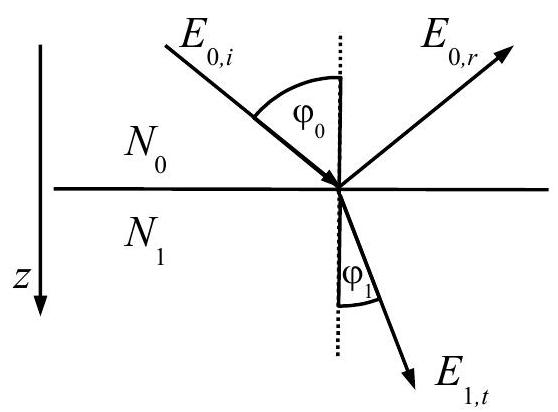
\includegraphics[width=0.8\linewidth, ]{obr1} 
		\caption{Odraz a průchod vlny na rozhraní dvou prostředí s indexem lomu $N_{0}$ a $N_{1}$.}
		\end{center}
		
	\end{figure} 
	V následujících výpočtech budeme také potřebovat inverzní situaci, kdy vlna dopadá z prostředí 1 do prostředí 0 , která je charakterizována koeficienty
	
	\begin{equation}
		r_{10}=\frac{N_{1}-N_{0}}{N_{1}+N_{0}}, \quad t_{10}=\frac{2 N_{1}}{N_{1}+N_{0}} 
	\end{equation}

	
	Jak lze dosazením lehce dokázat, mezi koeficienty (1) a (2) platí vztahy
	
	\begin{equation}
		r_{10}=-r_{01}, \quad t_{01} t_{10}+r_{01}^{2}=1.
	\end{equation}
	\subsubsection{Propustnost absorbující tlusté vrstvy}
	Propustnost $T_{012}$ vrstvy 1 z prostředí 0 do prostředí 2 je definována jako podíl prošlého záření $I_{2,t}$ a dopadajícího záření $I_{0,i}$:
	
	\begin{equation}
		T_{012} \equiv \frac{I_{2, t}}{I_{0, i}} 
	\end{equation}
	\subsubsection{Určení indexu lomu neabsorbující tlusté vrstvy z její propustnosti}
	V případě neabsorbujícího materiálu získáme hodnotu propustnosti užitím formule
	
	\begin{equation}
		T_{\mathrm{s}}=\frac{1-R_{01}}{1+R_{01}},
	\end{equation}
	kde $R_{01}$ je odrazivost - $R_{01} = |r_{01}^2|$. Po dosazení Fresnelových koeficientů (1) získáme formuli
	
	\begin{equation}
		T_{\mathrm{s}}=\frac{2 n_{0} n_{\mathrm{s}}}{n_{0}^{2}+n_{\mathrm{s}}^{2}},
	\end{equation}
	
	kde pomocí $N_{1}=n_{\mathrm{s}}$ je označen reálný index lomu tlusté vrstvy (substrátu). Dále budeme při  zpracování dat předpokládat, že index lomu prostředí je rovný vakuu a tedy $n_{0}=1$ a pro propustnost dostáváme
	
	\begin{equation}
		T_{\mathrm{s}}=\frac{2 n_{\mathrm{s}}}{1+n_{\mathrm{s}}^{2}}.
	\end{equation}
	
	Tato rovnice vede na kvadratickou rovnici pro $n_{\mathrm{s}}$ jejíz řešením je
	
	\begin{equation}
		n_{\mathrm{s}}(\lambda)=\frac{1+\sqrt{1-T_{\mathrm{s}}(\lambda)^{2}}}{T_{\mathrm{s}}(\lambda)}.
	\end{equation}
	Použitím této formule pro každou vlnovou délku $\lambda$ získáme hledaný index lomu $n_s(\lambda)$.
	\subsubsection{Cauchyova rovnice}
	Jedná se o jednu z nejjednodušších aproximací spektrální závislosti indexu lomu odpovídající oblasti bez absorpce:
	
	\begin{equation}
		n(\lambda)=A+\frac{B}{\lambda^{2}} 
	\end{equation}
	kde koeficient $A$ představuje dlouhovlnnou limitu indexu lomu (ze získaných dat se přesvědčíme, že funkce indexu lomu pro větší vlnové délky v podstatě konverguje k jisté hodnotě - koeficientu $A$). Koeficient $B$ vyjadřuje dispersi, tj závislost na vlnové délce. Jelikož v neabsorbující oblasti index lomu s klesající vlnovou délkou vždy roste,  je koeficient $B$ vždy kladný.
	
	\subsection{Určení indexu lomu a tloušťku tenké vrstvy}
	Tenká vrstva je vrstva dostatečně tenká na to, pro měřenou vlnovou délku docházelo k interferenci odražených paprsků od rozhraní. Jelikož je interference zásadně ovlivněna tloušťkou tenké vrstvy, je možné tloušťku zjistit ze samotné spektroskopické závislosti propustnosti. 
	
	Pro propustnost systému podložka-vrstva lze odvodit vztah:
	

{\small \begin{equation}
		T_{f}=\frac{4 n_{1}^{2} n}{n_{1}^{2}(n+1)^{2}-\left(n^{2}-n_{1}^{2}\right)\left(n_{1}^{2}-1\right) \sin ^{2}(x / 2)},
\end{equation}}
kde $x$ je fázový posun paprsků ve vrstvě. Při kolmém dopadu světla je dráhový rozdíl interferujících paprsků $s = 2n_1d$ a pro jejich fázový posun $x$ platí

\begin{equation}
	x=\frac{2 \pi}{\lambda} s \quad \text { nebo } \quad x=\frac{2 \pi}{\lambda} 2 n_{1} d
\end{equation}
Je tedy zřejmé, že se propustnost $T_f$ mění při změně vlnové délky dopadajícího světla a \textbf{pro jisté vlnové délky obdržíme maxima nebo minima propustnosti.}
Známe-li index lomu podložky $n$, index lomu tenké vrstvy stanovíme použitím formule 

\begin{equation}
	n_{1}=\frac{1 \pm \sqrt{1-T_{f}^{\min }}}{\sqrt{T_{f}^{\min }}} \sqrt{n}
\end{equation}

	Abychom mohli stanovit propustnost systému vrstva-podložka, zavedeme tzv. \textit{měřenou propustnost}
	\begin{equation}
		T_m = \frac {T_{fs}}{T_{ss}}
	\end{equation}
	kde $T_{ss}$ je propustnost samotné podložky a $T_{fs}$ propustnost podložky s vrstvou. Hledanou veličinu $T_f$ pak vypočteme ze vztahu
	
\begin{equation}
		T_{f}=T_{m} \frac{1-R_{s}}{1+R_{s}\left(1-T_{m}\right)}
\end{equation}
	
	kde
	\begin{equation}
		R_{s}=\frac {(n-1)^{2}}{(n+1)^{2}}
	\end{equation}
	Z grafu závislosti $T_m = f(\lambda)$ stanovíme \textit{minima} a pomocí formule (16) vypočítáme odpovídající hodnotu $T_f$. Pro vlnovou délku $\lambda$, pro kterou nastal tento extrém, stanovíme hledanou hodnotu indexu lomu $n_1$ vrstvy z rovnice (14).
	
	Pro určení tloušťky vrstvy použijeme formuli
	\begin{equation}
		d_1 = \frac{\lambda\lambda^\prime}{2(n_1^\prime \lambda-n_1\lambda^\prime)},
	\end{equation}
	kde $\lambda^\prime$ a $\lambda, \lambda^\prime < \lambda$ jsou vlnové délky dvou sousedních minim a $n^\prime, n$ hodnoty indexu lomu při těchto vlnových délkách. 
	
	\subsection{Lambert-Beerův zákon}
	Při průchodu monochromatické světelné vlny homogenní vrstvou látky o tloušťce $d$ za předpokladu zanedbatelné odrazivosti vedoucí k reflexním ztrátám je propustnost dána Lambert-Beerovým zákonem:	
	\begin{equation}
		T=\exp (-\alpha d)
	\end{equation}
	kde $\alpha$ je koeficient absorpce světla, který obecně závisí na vlnové délce dopadajícího záření. 
	\section{Měření}\subsection{Určení indexu lomu neabsorbující tlusté vrstvy z její propustnosti}	Pro vzorek skla BK7 získáme z měření následující závislost propustnosti na vlnové délce:	\begin{figure}[H]
	\begin{center}		
		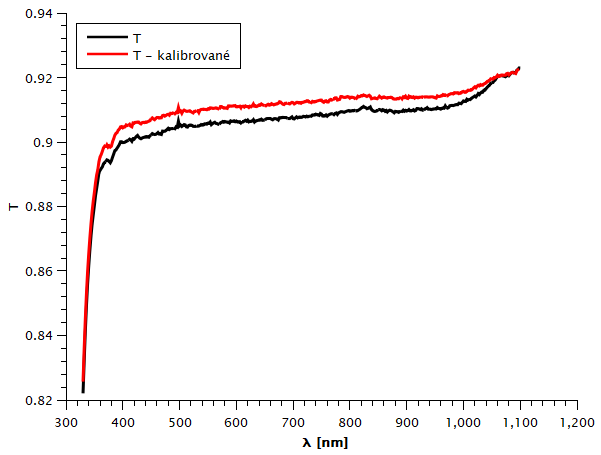
\includegraphics[width=0.75\linewidth, ]{propustnostbk72} 		
		\caption{Závislost propustnosti na vlnové délce pro sklo BK7 bez kalibrace a s kalibrací.}	\end{center}\end{figure} 
	Po aplikaci formule (8) získáme závislost indexu lomu na vlnové délce:
	\begin{figure}[H]
	\begin{center}		
		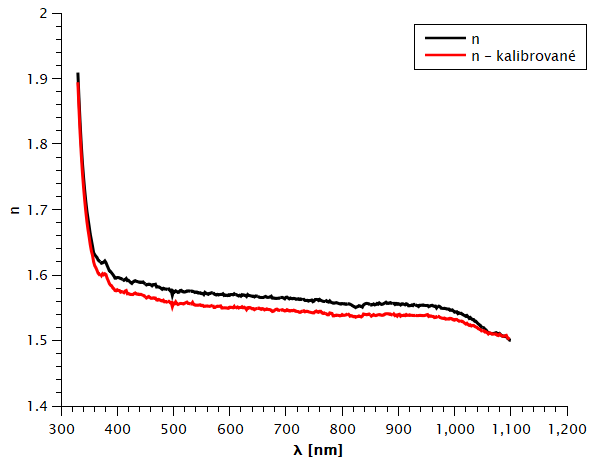
\includegraphics[width=0.75\linewidth, ]{bk7n2} 
		\caption{Závislost indexu lomu na vlnové délce pro sklo BK7}
	\end{center}
	\end{figure}
	kterou aproximujeme Cauchyovým vztahem:
	\begin{figure}[H]
		\begin{center}
			
			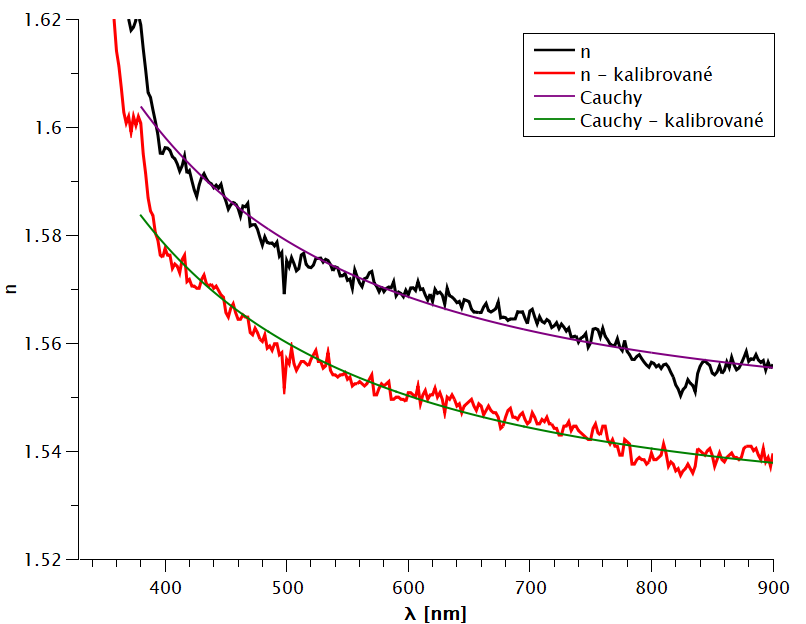
\includegraphics[width=0.8\linewidth, ]{cauchy} 
			\caption{Závislost indexu lomu na vlnové délce a její aproximace Cauchyovou rovnicí}
		\end{center}
	\end{figure}
	Po aproximaci získáváme koeficienty:
	{\small \begin{gather*}
		A=1.54493\pm 0.00035, B = (8.50 \pm 0.11).10^3\,\mathrm{nm^2}\\ 
		A_C = 1.52788\pm 0.00032, B_C = (8.05\pm 0.10).10^3\,\mathrm{nm^2}
	\end{gather*}}
	
	\subsection{Určení indexu lomu a tloušťky tenké vrstvy}
	Po měření získáváme hodnoty propustnosti pro substrát a tenkou vrstvu:
	\begin{figure}[H]
		\begin{center}
			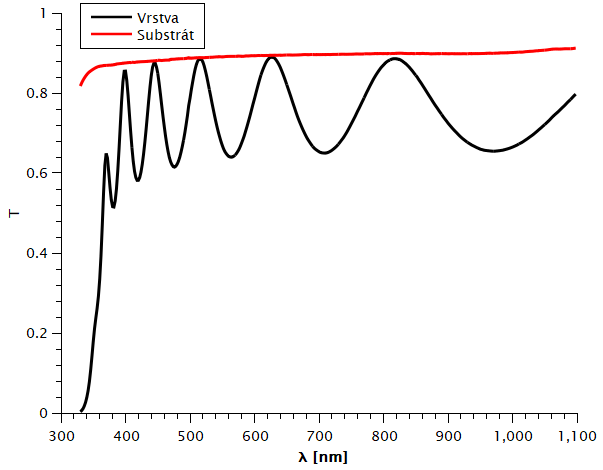
\includegraphics[width=0.8\linewidth, ]{tvrstvasubstrat} 
			\caption{Závislost propustnosti na vlnové délce pro tenkou vrstvu a substrát}	\end{center}\end{figure}
	Použitím formule (8) zjistíme index lomu substrátu $n$, který dále využijeme k výpočtu indexu lomu tenké vrstvy prostřednictvím formulí (17) ($R_s$) (15)($T_m$), a (16) ($T_f$), abychom byly schopni formulí (14) získat hodnotu indexu lomu tenké vrstvy $n_1$:
	
\begin{center}
		\begin{tabular}{|c|c|c|c|c|c|}
		\hline
		$\lambda$ & $n$      & $R_s$    & $T_m$    & $T_f$    & $n_1$  \\ \hline
		414       & 1.691 & 0.0659 & 0.689 & 0.631 & 3.312 \\ \hline
		476       & 1.658 & 0.0613 & 0.695 & 0.640 & 3.216 \\ \hline
		564       & 1.629 & 0.0573 & 0.717 & 0.665 & 3.028 \\ \hline
		710       & 1.612 & 0.0549 & 0.725 & 0.675 & 2.952 \\ \hline
		972       & 1.598 & 0.0530 & 0.728 & 0.679 & 2.915 \\ \hline
	\end{tabular}
\end{center}
	Získané hodnoty indexu lomu můžeme proložit v souladu s Cauchyho rovnicí, čímž získáme odhad spojité funkce indexu lomu na vlnové délce:
		\begin{figure}[H]
\begin{center}
		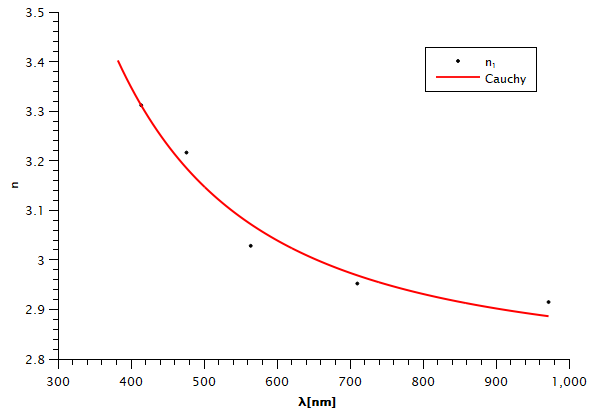
\includegraphics[width=0.8\linewidth, ]{tenkavrstvaaprox}
	\caption{Závislost indexu lomu na vlnové délce - aproximace Cauchyho rovnicí}
\end{center}
		\end{figure}
		
		Nalezená minima a získané indexy lomu tenké vrstvy použijeme k výpočtu její tloušťky pomocí formule (18):
		\begin{center}
			\begin{tabular}{|c|c|c|c|c|}
			\hline
			$\lambda $[nm] & $\lambda^\prime$ [nm] & n     & n$^\prime$    & d [nm]   \\ \hline
			414            & 476                   & 3.312 & 3.216 & 402.027  \\ \hline
			476            & 564                   & 3.216 & 3.028 & 360.3582 \\ \hline
			564            & 710                   & 3.028 & 2.952 & 412.8656 \\ \hline
			710            & 972                   & 2.952 & 2.915 & 431.49   \\ \hline
		\end{tabular}
		\end{center}
		\begin{equation*}
			d = (400 \pm 15) \,\rm nm
		\end{equation*}
		\subsection{Lambert-Beerův zákon}
		Měříme postupně spektrální propustnost jedné až čtyř vrstev stejného materiálu, jehož tloušťku jsme naměřili:
		
		\begin{center}
			\begin{center}
					\begin{tabular}{|c|c|}
				\hline
				d [mm] & n  \\ \hline
				3.4    & 1  \\ \hline
				3.45   & 12 \\ \hline
				3.5    & 9  \\ \hline
				3.6    & 4  \\ \hline
			\end{tabular}
			\end{center}
		\end{center}
	\begin{equation}
		d = 3.49 \pm 0.03 \,\rm mm
	\end{equation}
	Úpravou L-B zákona (formule (19)) získáme
	\begin{equation*}
		 {\ln T} = - \alpha d 
	\end{equation*}
	\begin{figure}[H]
	\begin{center}
		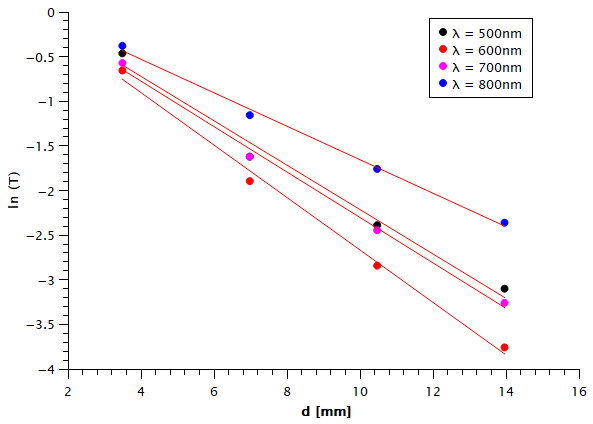
\includegraphics[width=0.8\linewidth, ]{lnfit}
		\caption{Závislost zlogaritmované hodnoty propustnosti na tloušťce vrstvy}
	\end{center}
	\end{figure}
	Získáváme hodnoty $\alpha$:
	{\small \begin{gather*}
		\alpha_{500} = 0.249\pm0.021\, \mathrm{m^{-1}} , \alpha_{600} = 0.294\pm-0.016\, \mathrm{m^{-1}}\\
		\alpha _{700} = 0.255 \pm 0.012\,\mathrm{m^{-1}}, \alpha_{800} = 0.188 \pm 0.009 \,\mathrm{m^{-1}}
	\end{gather*}}
	Pro ověření platnosti L-B zákona vizualizujeme závislost absorpčního koeficientu  $\alpha = - \frac{ln(T)}{d}$ na vlnové délce:
	\begin{figure}[H]
		\begin{center}
			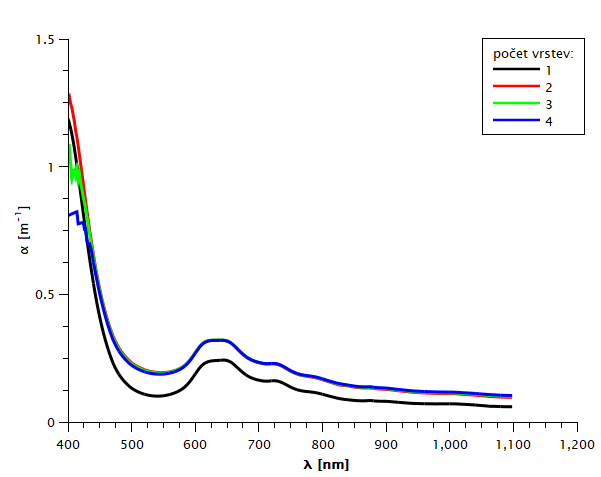
\includegraphics[width=0.8\linewidth, ]{alpha}
			\caption{Závislost hodnoty $\alpha$ na vlnové délce}
		\end{center}
	\end{figure}
	Kromě hodnoty pro pouze jednu vrstvu se křivky v intervalu $\lambda \in (400; 900) \,\rm$ shodují. Proto předpokládáme platnost L-B zákona pro tento interval, odchylka pouze jedné vrstvy může být způsobena skutečností, že tato vrstva se od vrstev ostatních značně odlišovala.\newpage
	
	
	\section{Závěr}
	Podařilo se nám určit spektrální závislost indexu lomu pro sklo BK7, pro tenkou vrstvu jsme kromě závislosti indexu lomu úspěšně změřili i její tloušťku a index lomu odhadli prostřednictvím Cauchyho rovnice. U ověření Lambert-Beerova zákona jsme se setkali s nevyhovujícími výsledky pro pouze jednu vrstvu, předpokládáme, že tato deviace pramení z rozdílných rozměrů oproti ostatním vrstvám.
	
	


	

	
	% Nakonec nezapomeňte projet text programem vlna nebo vlnka, např.
	% 	vlna -m -l -n mojeuloha.tex
	% nebo zkontrolovat a opravit jednopísmenné předložky na koncích řádků ručně.
\end{multicols}
\end{document}
